\documentclass[landscape]{article}
\usepackage[a4paper, margin=2cm]{geometry}
\usepackage{tikz}
\usetikzlibrary{shapes,arrows,positioning,fit,backgrounds,calc,shadows}

\begin{document}

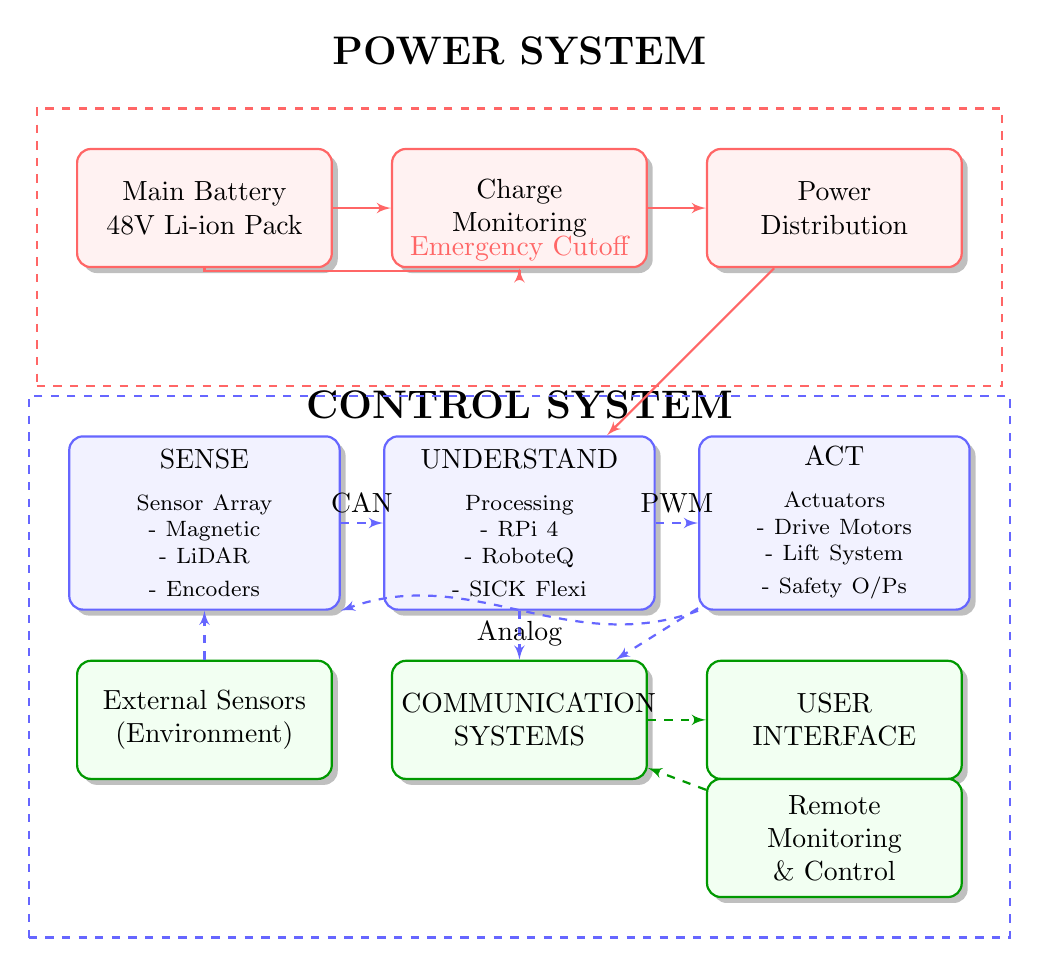
\begin{tikzpicture}[
    % Define better-looking styles
    powerblock/.style={
        rectangle,
        draw=red!60,
        thick,
        fill=red!5,
        text width=3cm,
        minimum height=1.5cm,
        align=center,
        rounded corners=5pt,
        drop shadow
    },
    controlblock/.style={
        rectangle,
        draw=blue!60,
        thick,
        fill=blue!5,
        text width=3.2cm,
        minimum height=2.2cm,
        align=center,
        rounded corners=5pt,
        drop shadow
    },
    commblock/.style={
        rectangle,
        draw=green!60!black,
        thick,
        fill=green!5,
        text width=3cm,
        minimum height=1.5cm,
        align=center,
        rounded corners=5pt,
        drop shadow
    },
    line/.style={-latex', thick},
    powerline/.style={draw=red!60, -latex', thick},
    dataline/.style={draw=blue!60, dashed, -latex', thick},
    commline/.style={draw=green!60!black, dashed, -latex', thick}
]

% Title
\node[font=\Large\bfseries] at (0,5) {POWER SYSTEM};

% Power System
\begin{scope}
    \node[powerblock] (battery) at (-4,3) {Main Battery\\48V Li-ion Pack};
    \node[powerblock] (monitoring) at (0,3) {Charge\\Monitoring};
    \node[powerblock] (distribution) at (4,3) {Power\\Distribution};
    
    % Power connections
    \draw[powerline] (battery) -- (monitoring);
    \draw[powerline] (monitoring) -- (distribution);
    \draw[powerline, red!60] (battery) -- ++(0,-0.8) -| node[above] {Emergency Cutoff} (monitoring);
    
    % Power system boundary
    \node[draw=red!60, dashed, thick, fit={(battery) (distribution) ($(battery.south)+(0,-1)$)}, 
          inner sep=0.5cm] (power_boundary) {};
\end{scope}

% Control System Title
\node[font=\Large\bfseries] at (0,0.5) {CONTROL SYSTEM};

% Main Control Blocks
\node[controlblock] (sense) at (-4,-1) {SENSE\\[0.2cm]
    \footnotesize
    Sensor Array\\
    - Magnetic\\
    - LiDAR\\
    - Encoders};

\node[controlblock] (understand) at (0,-1) {UNDERSTAND\\[0.2cm]
    \footnotesize
    Processing\\
    - RPi 4\\
    - RoboteQ\\
    - SICK Flexi};

\node[controlblock] (act) at (4,-1) {ACT\\[0.2cm]
    \footnotesize
    Actuators\\
    - Drive Motors\\
    - Lift System\\
    - Safety O/Ps};

% Communication Blocks
\node[commblock] (comm) at (0,-3.5) {COMMUNICATION\\SYSTEMS};
\node[commblock] (ui) at (4,-3.5) {USER\\INTERFACE};

% External Blocks
\node[commblock] (ext_sensors) at (-4,-3.5) {External Sensors\\(Environment)};
\node[commblock] (remote) at (4,-5) {Remote Monitoring\\{\&} Control};

% Control system boundary
\node[draw=blue!60, dashed, thick, fit={(sense) (act) (ext_sensors) (remote)}, 
      inner sep=0.5cm] (control_boundary) {};

% Connections
\draw[powerline] (distribution) -- (understand);
\draw[dataline] (sense) -- node[above] {CAN} (understand);
\draw[dataline] (understand) -- node[above] {PWM} (act);
\draw[dataline] (understand) -- (comm);
\draw[dataline] (act) -- (comm);
\draw[commline] (comm) -- (ui);
\draw[dataline] (ext_sensors) -- (sense);
\draw[commline] (remote) -- (comm);

% Feedback loops
\draw[dataline] (act.south west) to[out=200, in=20] 
    node[below, text width=2cm, align=center] {Analog} (sense.south east);

\end{tikzpicture}

\end{document} 